% SOURCE: edit-harness/results/frame_a/cells/cell_*_real_MIX_{A,B,C}_*.json
% !TEX encoding = UTF-8 Unicode
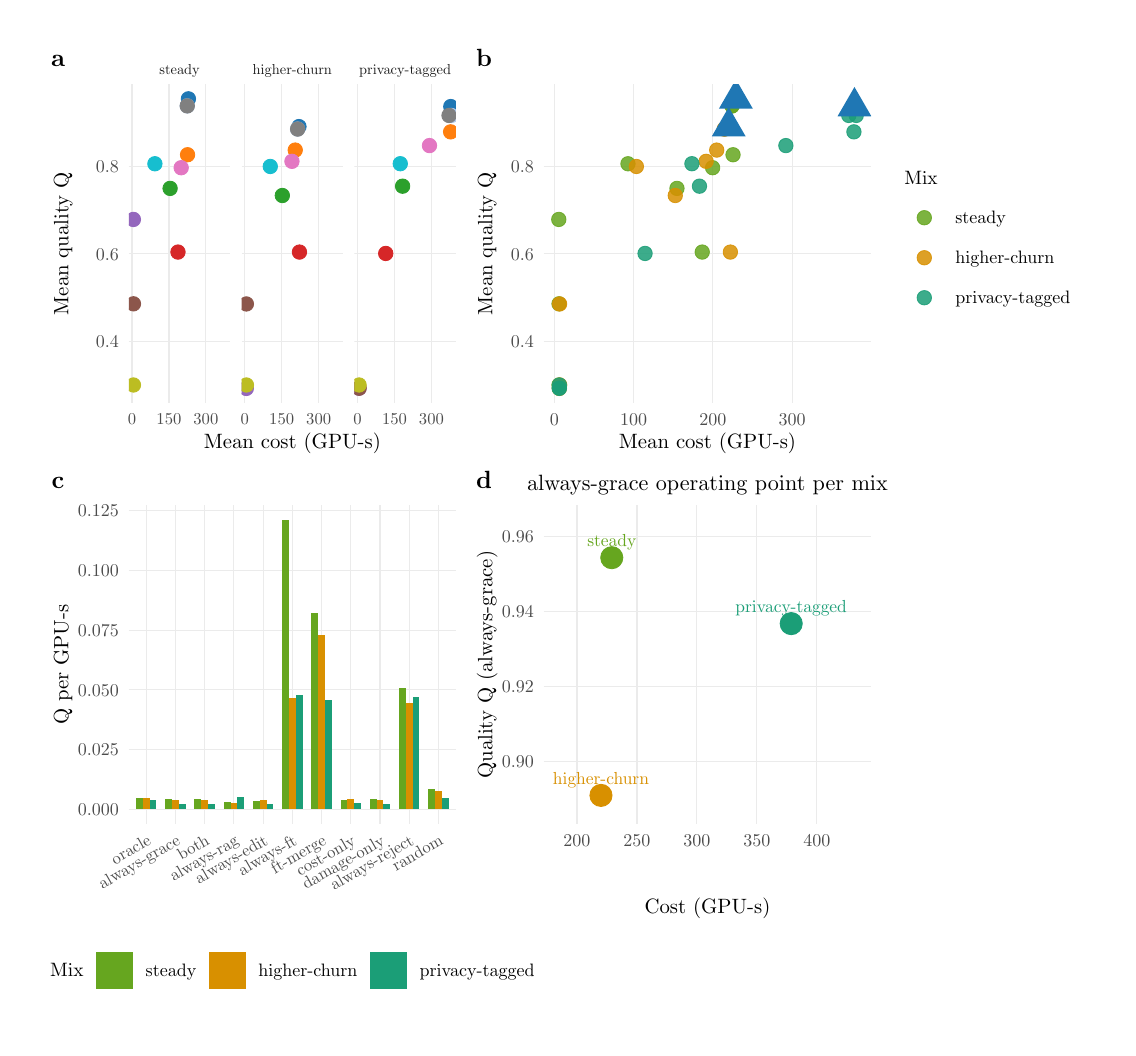
\begin{tikzpicture}[x=1pt,y=1pt]
\definecolor{fillColor}{RGB}{255,255,255}
\path[use as bounding box,fill=fillColor,fill opacity=0.00] (0,0) rectangle (390.26,361.35);
\begin{scope}
\path[clip] (  0.00,  0.00) rectangle (390.26,361.35);
\definecolor{drawColor}{RGB}{255,255,255}
\definecolor{fillColor}{RGB}{255,255,255}

\path[draw=drawColor,line width= 0.6pt,line join=round,line cap=round,fill=fillColor] (  0.00,  0.00) rectangle (390.26,361.35);
\end{scope}
\begin{scope}
\path[clip] (  5.50,203.79) rectangle (158.76,355.85);
\definecolor{fillColor}{RGB}{255,255,255}

\path[fill=fillColor] (  5.50,203.79) rectangle (158.76,355.85);
\end{scope}
\begin{scope}
\path[clip] (158.76,203.79) rectangle (384.76,355.85);
\definecolor{fillColor}{RGB}{255,255,255}

\path[fill=fillColor] (158.76,203.79) rectangle (384.76,355.85);
\end{scope}
\begin{scope}
\path[clip] (  5.50,  5.50) rectangle (158.76,203.79);
\definecolor{fillColor}{RGB}{255,255,255}

\path[fill=fillColor] (  5.50,  5.50) rectangle (158.76,203.79);
\end{scope}
\begin{scope}
\path[clip] (158.76,  5.50) rectangle (384.76,203.79);
\definecolor{fillColor}{RGB}{255,255,255}

\path[fill=fillColor] (158.76,  5.50) rectangle (384.76,203.79);
\end{scope}
\begin{scope}
\path[clip] ( 36.53,225.75) rectangle ( 73.27,340.86);
\definecolor{drawColor}{gray}{0.92}

\path[draw=drawColor,line width= 0.4pt,line join=round] ( 36.53,248.03) --
	( 73.27,248.03);

\path[draw=drawColor,line width= 0.4pt,line join=round] ( 36.53,279.63) --
	( 73.27,279.63);

\path[draw=drawColor,line width= 0.4pt,line join=round] ( 36.53,311.23) --
	( 73.27,311.23);

\path[draw=drawColor,line width= 0.4pt,line join=round] ( 37.70,225.75) --
	( 37.70,340.86);

\path[draw=drawColor,line width= 0.4pt,line join=round] ( 51.05,225.75) --
	( 51.05,340.86);

\path[draw=drawColor,line width= 0.4pt,line join=round] ( 64.40,225.75) --
	( 64.40,340.86);
\definecolor{drawColor}{RGB}{44,160,44}
\definecolor{fillColor}{RGB}{44,160,44}

\path[draw=drawColor,line width= 0.3pt,line join=round,line cap=round,fill=fillColor] ( 51.47,303.27) circle (  2.61);
\definecolor{drawColor}{RGB}{31,119,180}
\definecolor{fillColor}{RGB}{31,119,180}

\path[draw=drawColor,line width= 0.3pt,line join=round,line cap=round,fill=fillColor] ( 58.08,335.63) circle (  2.61);
\definecolor{drawColor}{RGB}{174,199,232}
\definecolor{fillColor}{RGB}{174,199,232}

\path[draw=drawColor,line width= 0.3pt,line join=round,line cap=round,fill=fillColor] ( 57.65,333.08) circle (  2.61);
\definecolor{drawColor}{RGB}{214,39,40}
\definecolor{fillColor}{RGB}{214,39,40}

\path[draw=drawColor,line width= 0.3pt,line join=round,line cap=round,fill=fillColor] ( 54.31,280.26) circle (  2.61);
\definecolor{drawColor}{RGB}{255,127,14}
\definecolor{fillColor}{RGB}{255,127,14}

\path[draw=drawColor,line width= 0.3pt,line join=round,line cap=round,fill=fillColor] ( 57.77,315.43) circle (  2.61);
\definecolor{drawColor}{RGB}{148,103,189}
\definecolor{fillColor}{RGB}{148,103,189}

\path[draw=drawColor,line width= 0.3pt,line join=round,line cap=round,fill=fillColor] ( 38.20,292.05) circle (  2.61);
\definecolor{drawColor}{RGB}{140,86,75}
\definecolor{fillColor}{RGB}{140,86,75}

\path[draw=drawColor,line width= 0.3pt,line join=round,line cap=round,fill=fillColor] ( 38.22,261.56) circle (  2.61);
\definecolor{drawColor}{RGB}{227,119,194}
\definecolor{fillColor}{RGB}{227,119,194}

\path[draw=drawColor,line width= 0.3pt,line join=round,line cap=round,fill=fillColor] ( 55.47,310.74) circle (  2.61);
\definecolor{drawColor}{gray}{0.50}
\definecolor{fillColor}{gray}{0.50}

\path[draw=drawColor,line width= 0.3pt,line join=round,line cap=round,fill=fillColor] ( 57.66,333.08) circle (  2.61);
\definecolor{drawColor}{RGB}{188,189,34}
\definecolor{fillColor}{RGB}{188,189,34}

\path[draw=drawColor,line width= 0.3pt,line join=round,line cap=round,fill=fillColor] ( 38.22,232.23) circle (  2.61);
\definecolor{drawColor}{RGB}{23,190,207}
\definecolor{fillColor}{RGB}{23,190,207}

\path[draw=drawColor,line width= 0.3pt,line join=round,line cap=round,fill=fillColor] ( 45.97,312.17) circle (  2.61);
\end{scope}
\begin{scope}
\path[clip] ( 77.27,225.75) rectangle (114.01,340.86);
\definecolor{drawColor}{gray}{0.92}

\path[draw=drawColor,line width= 0.4pt,line join=round] ( 77.27,248.03) --
	(114.01,248.03);

\path[draw=drawColor,line width= 0.4pt,line join=round] ( 77.27,279.63) --
	(114.01,279.63);

\path[draw=drawColor,line width= 0.4pt,line join=round] ( 77.27,311.23) --
	(114.01,311.23);

\path[draw=drawColor,line width= 0.4pt,line join=round] ( 78.44,225.75) --
	( 78.44,340.86);

\path[draw=drawColor,line width= 0.4pt,line join=round] ( 91.79,225.75) --
	( 91.79,340.86);

\path[draw=drawColor,line width= 0.4pt,line join=round] (105.15,225.75) --
	(105.15,340.86);
\definecolor{drawColor}{RGB}{44,160,44}
\definecolor{fillColor}{RGB}{44,160,44}

\path[draw=drawColor,line width= 0.3pt,line join=round,line cap=round,fill=fillColor] ( 92.02,300.70) circle (  2.61);
\definecolor{drawColor}{RGB}{31,119,180}
\definecolor{fillColor}{RGB}{31,119,180}

\path[draw=drawColor,line width= 0.3pt,line join=round,line cap=round,fill=fillColor] ( 98.03,325.60) circle (  2.61);
\definecolor{drawColor}{RGB}{174,199,232}
\definecolor{fillColor}{RGB}{174,199,232}

\path[draw=drawColor,line width= 0.3pt,line join=round,line cap=round,fill=fillColor] ( 97.52,324.71) circle (  2.61);
\definecolor{drawColor}{RGB}{214,39,40}
\definecolor{fillColor}{RGB}{214,39,40}

\path[draw=drawColor,line width= 0.3pt,line join=round,line cap=round,fill=fillColor] ( 98.21,280.26) circle (  2.61);
\definecolor{drawColor}{RGB}{255,127,14}
\definecolor{fillColor}{RGB}{255,127,14}

\path[draw=drawColor,line width= 0.3pt,line join=round,line cap=round,fill=fillColor] ( 96.68,317.11) circle (  2.61);
\definecolor{drawColor}{RGB}{148,103,189}
\definecolor{fillColor}{RGB}{148,103,189}

\path[draw=drawColor,line width= 0.3pt,line join=round,line cap=round,fill=fillColor] ( 79.00,230.99) circle (  2.61);
\definecolor{drawColor}{RGB}{140,86,75}
\definecolor{fillColor}{RGB}{140,86,75}

\path[draw=drawColor,line width= 0.3pt,line join=round,line cap=round,fill=fillColor] ( 79.03,261.51) circle (  2.61);
\definecolor{drawColor}{RGB}{227,119,194}
\definecolor{fillColor}{RGB}{227,119,194}

\path[draw=drawColor,line width= 0.3pt,line join=round,line cap=round,fill=fillColor] ( 95.49,313.05) circle (  2.61);
\definecolor{drawColor}{gray}{0.50}
\definecolor{fillColor}{gray}{0.50}

\path[draw=drawColor,line width= 0.3pt,line join=round,line cap=round,fill=fillColor] ( 97.55,324.71) circle (  2.61);
\definecolor{drawColor}{RGB}{188,189,34}
\definecolor{fillColor}{RGB}{188,189,34}

\path[draw=drawColor,line width= 0.3pt,line join=round,line cap=round,fill=fillColor] ( 79.04,232.23) circle (  2.61);
\definecolor{drawColor}{RGB}{23,190,207}
\definecolor{fillColor}{RGB}{23,190,207}

\path[draw=drawColor,line width= 0.3pt,line join=round,line cap=round,fill=fillColor] ( 87.66,311.19) circle (  2.61);
\end{scope}
\begin{scope}
\path[clip] (118.01,225.75) rectangle (154.76,340.86);
\definecolor{drawColor}{gray}{0.92}

\path[draw=drawColor,line width= 0.4pt,line join=round] (118.01,248.03) --
	(154.76,248.03);

\path[draw=drawColor,line width= 0.4pt,line join=round] (118.01,279.63) --
	(154.76,279.63);

\path[draw=drawColor,line width= 0.4pt,line join=round] (118.01,311.23) --
	(154.76,311.23);

\path[draw=drawColor,line width= 0.4pt,line join=round] (119.19,225.75) --
	(119.19,340.86);

\path[draw=drawColor,line width= 0.4pt,line join=round] (132.54,225.75) --
	(132.54,340.86);

\path[draw=drawColor,line width= 0.4pt,line join=round] (145.89,225.75) --
	(145.89,340.86);
\definecolor{drawColor}{RGB}{44,160,44}
\definecolor{fillColor}{RGB}{44,160,44}

\path[draw=drawColor,line width= 0.3pt,line join=round,line cap=round,fill=fillColor] (135.48,304.07) circle (  2.61);
\definecolor{drawColor}{RGB}{31,119,180}
\definecolor{fillColor}{RGB}{31,119,180}

\path[draw=drawColor,line width= 0.3pt,line join=round,line cap=round,fill=fillColor] (152.89,332.84) circle (  2.61);
\definecolor{drawColor}{RGB}{174,199,232}
\definecolor{fillColor}{RGB}{174,199,232}

\path[draw=drawColor,line width= 0.3pt,line join=round,line cap=round,fill=fillColor] (153.09,329.63) circle (  2.61);
\definecolor{drawColor}{RGB}{214,39,40}
\definecolor{fillColor}{RGB}{214,39,40}

\path[draw=drawColor,line width= 0.3pt,line join=round,line cap=round,fill=fillColor] (129.38,279.76) circle (  2.61);
\definecolor{drawColor}{RGB}{255,127,14}
\definecolor{fillColor}{RGB}{255,127,14}

\path[draw=drawColor,line width= 0.3pt,line join=round,line cap=round,fill=fillColor] (152.83,323.70) circle (  2.61);
\definecolor{drawColor}{RGB}{148,103,189}
\definecolor{fillColor}{RGB}{148,103,189}

\path[draw=drawColor,line width= 0.3pt,line join=round,line cap=round,fill=fillColor] (119.73,231.07) circle (  2.61);
\definecolor{drawColor}{RGB}{140,86,75}
\definecolor{fillColor}{RGB}{140,86,75}

\path[draw=drawColor,line width= 0.3pt,line join=round,line cap=round,fill=fillColor] (119.76,231.07) circle (  2.61);
\definecolor{drawColor}{RGB}{227,119,194}
\definecolor{fillColor}{RGB}{227,119,194}

\path[draw=drawColor,line width= 0.3pt,line join=round,line cap=round,fill=fillColor] (145.19,318.74) circle (  2.61);
\definecolor{drawColor}{gray}{0.50}
\definecolor{fillColor}{gray}{0.50}

\path[draw=drawColor,line width= 0.3pt,line join=round,line cap=round,fill=fillColor] (152.25,329.63) circle (  2.61);
\definecolor{drawColor}{RGB}{188,189,34}
\definecolor{fillColor}{RGB}{188,189,34}

\path[draw=drawColor,line width= 0.3pt,line join=round,line cap=round,fill=fillColor] (119.76,232.23) circle (  2.61);
\definecolor{drawColor}{RGB}{23,190,207}
\definecolor{fillColor}{RGB}{23,190,207}

\path[draw=drawColor,line width= 0.3pt,line join=round,line cap=round,fill=fillColor] (134.64,312.19) circle (  2.61);
\end{scope}
\begin{scope}
\path[clip] (  0.00,  0.00) rectangle (390.26,361.35);
\definecolor{drawColor}{gray}{0.10}

\node[text=drawColor,anchor=base,inner sep=0pt, outer sep=0pt, scale=  0.52] at ( 54.90,344.56) {steady};
\end{scope}
\begin{scope}
\path[clip] (  0.00,  0.00) rectangle (390.26,361.35);
\definecolor{drawColor}{gray}{0.10}

\node[text=drawColor,anchor=base,inner sep=0pt, outer sep=0pt, scale=  0.52] at ( 95.64,344.56) {higher-churn};
\end{scope}
\begin{scope}
\path[clip] (  0.00,  0.00) rectangle (390.26,361.35);
\definecolor{drawColor}{gray}{0.10}

\node[text=drawColor,anchor=base,inner sep=0pt, outer sep=0pt, scale=  0.52] at (136.39,344.56) {privacy-tagged};
\end{scope}
\begin{scope}
\path[clip] (  0.00,  0.00) rectangle (390.26,361.35);
\definecolor{drawColor}{gray}{0.30}

\node[text=drawColor,anchor=base,inner sep=0pt, outer sep=0pt, scale=  0.60] at ( 37.70,218.02) {0};

\node[text=drawColor,anchor=base,inner sep=0pt, outer sep=0pt, scale=  0.60] at ( 51.05,218.02) {150};

\node[text=drawColor,anchor=base,inner sep=0pt, outer sep=0pt, scale=  0.60] at ( 64.40,218.02) {300};
\end{scope}
\begin{scope}
\path[clip] (  0.00,  0.00) rectangle (390.26,361.35);
\definecolor{drawColor}{gray}{0.30}

\node[text=drawColor,anchor=base,inner sep=0pt, outer sep=0pt, scale=  0.60] at ( 78.44,218.02) {0};

\node[text=drawColor,anchor=base,inner sep=0pt, outer sep=0pt, scale=  0.60] at ( 91.79,218.02) {150};

\node[text=drawColor,anchor=base,inner sep=0pt, outer sep=0pt, scale=  0.60] at (105.15,218.02) {300};
\end{scope}
\begin{scope}
\path[clip] (  0.00,  0.00) rectangle (390.26,361.35);
\definecolor{drawColor}{gray}{0.30}

\node[text=drawColor,anchor=base,inner sep=0pt, outer sep=0pt, scale=  0.60] at (119.19,218.02) {0};

\node[text=drawColor,anchor=base,inner sep=0pt, outer sep=0pt, scale=  0.60] at (132.54,218.02) {150};

\node[text=drawColor,anchor=base,inner sep=0pt, outer sep=0pt, scale=  0.60] at (145.89,218.02) {300};
\end{scope}
\begin{scope}
\path[clip] (  0.00,  0.00) rectangle (390.26,361.35);
\definecolor{drawColor}{gray}{0.30}

\node[text=drawColor,anchor=base east,inner sep=0pt, outer sep=0pt, scale=  0.65] at ( 32.93,245.79) {0.4};

\node[text=drawColor,anchor=base east,inner sep=0pt, outer sep=0pt, scale=  0.65] at ( 32.93,277.39) {0.6};

\node[text=drawColor,anchor=base east,inner sep=0pt, outer sep=0pt, scale=  0.65] at ( 32.93,308.99) {0.8};
\end{scope}
\begin{scope}
\path[clip] (  0.00,  0.00) rectangle (390.26,361.35);
\definecolor{drawColor}{RGB}{0,0,0}

\node[text=drawColor,anchor=base,inner sep=0pt, outer sep=0pt, scale=  0.75] at ( 95.64,209.25) {Mean cost (GPU-s)};
\end{scope}
\begin{scope}
\path[clip] (  0.00,  0.00) rectangle (390.26,361.35);
\definecolor{drawColor}{RGB}{0,0,0}

\node[text=drawColor,rotate= 90.00,anchor=base,inner sep=0pt, outer sep=0pt, scale=  0.75] at ( 14.67,283.31) {Mean quality Q};
\end{scope}
\begin{scope}
\path[clip] (  0.00,  0.00) rectangle (390.26,361.35);
\definecolor{drawColor}{RGB}{0,0,0}

\node[text=drawColor,anchor=base,inner sep=0pt, outer sep=0pt, scale=  0.90] at ( 10.95,347.30) {\bfseries a};
\end{scope}
\begin{scope}
\path[clip] (186.53,225.75) rectangle (304.77,340.86);
\definecolor{drawColor}{gray}{0.92}

\path[draw=drawColor,line width= 0.4pt,line join=round] (186.53,248.03) --
	(304.77,248.03);

\path[draw=drawColor,line width= 0.4pt,line join=round] (186.53,279.63) --
	(304.77,279.63);

\path[draw=drawColor,line width= 0.4pt,line join=round] (186.53,311.23) --
	(304.77,311.23);

\path[draw=drawColor,line width= 0.4pt,line join=round] (190.30,225.75) --
	(190.30,340.86);

\path[draw=drawColor,line width= 0.4pt,line join=round] (218.95,225.75) --
	(218.95,340.86);

\path[draw=drawColor,line width= 0.4pt,line join=round] (247.60,225.75) --
	(247.60,340.86);

\path[draw=drawColor,line width= 0.4pt,line join=round] (276.24,225.75) --
	(276.24,340.86);
\definecolor{drawColor}{RGB}{102,166,31}
\definecolor{fillColor}{RGB}{102,166,31}

\path[draw=drawColor,draw opacity=0.85,line width= 0.3pt,line join=round,line cap=round,fill=fillColor,fill opacity=0.85] (234.62,303.27) circle (  2.61);

\path[draw=drawColor,draw opacity=0.85,line width= 0.3pt,line join=round,line cap=round,fill=fillColor,fill opacity=0.85] (255.91,335.63) circle (  2.61);

\path[draw=drawColor,draw opacity=0.85,line width= 0.3pt,line join=round,line cap=round,fill=fillColor,fill opacity=0.85] (254.49,333.08) circle (  2.61);

\path[draw=drawColor,draw opacity=0.85,line width= 0.3pt,line join=round,line cap=round,fill=fillColor,fill opacity=0.85] (243.75,280.26) circle (  2.61);

\path[draw=drawColor,draw opacity=0.85,line width= 0.3pt,line join=round,line cap=round,fill=fillColor,fill opacity=0.85] (254.88,315.43) circle (  2.61);

\path[draw=drawColor,draw opacity=0.85,line width= 0.3pt,line join=round,line cap=round,fill=fillColor,fill opacity=0.85] (191.91,292.05) circle (  2.61);

\path[draw=drawColor,draw opacity=0.85,line width= 0.3pt,line join=round,line cap=round,fill=fillColor,fill opacity=0.85] (192.00,261.56) circle (  2.61);

\path[draw=drawColor,draw opacity=0.85,line width= 0.3pt,line join=round,line cap=round,fill=fillColor,fill opacity=0.85] (247.50,310.74) circle (  2.61);

\path[draw=drawColor,draw opacity=0.85,line width= 0.3pt,line join=round,line cap=round,fill=fillColor,fill opacity=0.85] (254.55,333.08) circle (  2.61);

\path[draw=drawColor,draw opacity=0.85,line width= 0.3pt,line join=round,line cap=round,fill=fillColor,fill opacity=0.85] (191.99,232.23) circle (  2.61);

\path[draw=drawColor,draw opacity=0.85,line width= 0.3pt,line join=round,line cap=round,fill=fillColor,fill opacity=0.85] (216.92,312.17) circle (  2.61);
\definecolor{drawColor}{RGB}{216,144,0}
\definecolor{fillColor}{RGB}{216,144,0}

\path[draw=drawColor,draw opacity=0.85,line width= 0.3pt,line join=round,line cap=round,fill=fillColor,fill opacity=0.85] (234.00,300.70) circle (  2.61);

\path[draw=drawColor,draw opacity=0.85,line width= 0.3pt,line join=round,line cap=round,fill=fillColor,fill opacity=0.85] (253.33,325.60) circle (  2.61);

\path[draw=drawColor,draw opacity=0.85,line width= 0.3pt,line join=round,line cap=round,fill=fillColor,fill opacity=0.85] (251.71,324.71) circle (  2.61);

\path[draw=drawColor,draw opacity=0.85,line width= 0.3pt,line join=round,line cap=round,fill=fillColor,fill opacity=0.85] (253.92,280.26) circle (  2.61);

\path[draw=drawColor,draw opacity=0.85,line width= 0.3pt,line join=round,line cap=round,fill=fillColor,fill opacity=0.85] (248.98,317.11) circle (  2.61);

\path[draw=drawColor,draw opacity=0.85,line width= 0.3pt,line join=round,line cap=round,fill=fillColor,fill opacity=0.85] (192.10,230.99) circle (  2.61);

\path[draw=drawColor,draw opacity=0.85,line width= 0.3pt,line join=round,line cap=round,fill=fillColor,fill opacity=0.85] (192.21,261.51) circle (  2.61);

\path[draw=drawColor,draw opacity=0.85,line width= 0.3pt,line join=round,line cap=round,fill=fillColor,fill opacity=0.85] (245.16,313.05) circle (  2.61);

\path[draw=drawColor,draw opacity=0.85,line width= 0.3pt,line join=round,line cap=round,fill=fillColor,fill opacity=0.85] (251.80,324.71) circle (  2.61);

\path[draw=drawColor,draw opacity=0.85,line width= 0.3pt,line join=round,line cap=round,fill=fillColor,fill opacity=0.85] (192.23,232.23) circle (  2.61);

\path[draw=drawColor,draw opacity=0.85,line width= 0.3pt,line join=round,line cap=round,fill=fillColor,fill opacity=0.85] (219.95,311.19) circle (  2.61);
\definecolor{drawColor}{RGB}{27,158,119}
\definecolor{fillColor}{RGB}{27,158,119}

\path[draw=drawColor,draw opacity=0.85,line width= 0.3pt,line join=round,line cap=round,fill=fillColor,fill opacity=0.85] (242.75,304.07) circle (  2.61);

\path[draw=drawColor,draw opacity=0.85,line width= 0.3pt,line join=round,line cap=round,fill=fillColor,fill opacity=0.85] (298.76,332.84) circle (  2.61);

\path[draw=drawColor,draw opacity=0.85,line width= 0.3pt,line join=round,line cap=round,fill=fillColor,fill opacity=0.85] (299.39,329.63) circle (  2.61);

\path[draw=drawColor,draw opacity=0.85,line width= 0.3pt,line join=round,line cap=round,fill=fillColor,fill opacity=0.85] (223.09,279.76) circle (  2.61);

\path[draw=drawColor,draw opacity=0.85,line width= 0.3pt,line join=round,line cap=round,fill=fillColor,fill opacity=0.85] (298.56,323.70) circle (  2.61);

\path[draw=drawColor,draw opacity=0.85,line width= 0.3pt,line join=round,line cap=round,fill=fillColor,fill opacity=0.85] (192.06,231.07) circle (  2.61);

\path[draw=drawColor,draw opacity=0.85,line width= 0.3pt,line join=round,line cap=round,fill=fillColor,fill opacity=0.85] (192.14,231.07) circle (  2.61);

\path[draw=drawColor,draw opacity=0.85,line width= 0.3pt,line join=round,line cap=round,fill=fillColor,fill opacity=0.85] (273.97,318.74) circle (  2.61);

\path[draw=drawColor,draw opacity=0.85,line width= 0.3pt,line join=round,line cap=round,fill=fillColor,fill opacity=0.85] (296.70,329.63) circle (  2.61);

\path[draw=drawColor,draw opacity=0.85,line width= 0.3pt,line join=round,line cap=round,fill=fillColor,fill opacity=0.85] (192.14,232.23) circle (  2.61);

\path[draw=drawColor,draw opacity=0.85,line width= 0.3pt,line join=round,line cap=round,fill=fillColor,fill opacity=0.85] (240.02,312.19) circle (  2.61);
\definecolor{fillColor}{RGB}{31,119,180}

\path[fill=fillColor] (255.91,342.69) --
	(262.02,332.09) --
	(249.79,332.09) --
	cycle;

\path[fill=fillColor] (253.33,332.66) --
	(259.44,322.06) --
	(247.21,322.06) --
	cycle;

\path[fill=fillColor] (298.76,339.91) --
	(304.88,329.31) --
	(292.64,329.31) --
	cycle;
\end{scope}
\begin{scope}
\path[clip] (  0.00,  0.00) rectangle (390.26,361.35);
\definecolor{drawColor}{gray}{0.30}

\node[text=drawColor,anchor=base east,inner sep=0pt, outer sep=0pt, scale=  0.65] at (182.93,245.79) {0.4};

\node[text=drawColor,anchor=base east,inner sep=0pt, outer sep=0pt, scale=  0.65] at (182.93,277.39) {0.6};

\node[text=drawColor,anchor=base east,inner sep=0pt, outer sep=0pt, scale=  0.65] at (182.93,308.99) {0.8};
\end{scope}
\begin{scope}
\path[clip] (  0.00,  0.00) rectangle (390.26,361.35);
\definecolor{drawColor}{gray}{0.30}

\node[text=drawColor,anchor=base,inner sep=0pt, outer sep=0pt, scale=  0.65] at (190.30,217.68) {0};

\node[text=drawColor,anchor=base,inner sep=0pt, outer sep=0pt, scale=  0.65] at (218.95,217.68) {100};

\node[text=drawColor,anchor=base,inner sep=0pt, outer sep=0pt, scale=  0.65] at (247.60,217.68) {200};

\node[text=drawColor,anchor=base,inner sep=0pt, outer sep=0pt, scale=  0.65] at (276.24,217.68) {300};
\end{scope}
\begin{scope}
\path[clip] (  0.00,  0.00) rectangle (390.26,361.35);
\definecolor{drawColor}{RGB}{0,0,0}

\node[text=drawColor,anchor=base,inner sep=0pt, outer sep=0pt, scale=  0.75] at (245.65,209.25) {Mean cost (GPU-s)};
\end{scope}
\begin{scope}
\path[clip] (  0.00,  0.00) rectangle (390.26,361.35);
\definecolor{drawColor}{RGB}{0,0,0}

\node[text=drawColor,rotate= 90.00,anchor=base,inner sep=0pt, outer sep=0pt, scale=  0.75] at (167.92,283.31) {Mean quality Q};
\end{scope}
\begin{scope}
\path[clip] (  0.00,  0.00) rectangle (390.26,361.35);
\definecolor{drawColor}{RGB}{0,0,0}

\node[text=drawColor,anchor=base west,inner sep=0pt, outer sep=0pt, scale=  0.70] at (316.77,304.58) {Mix};
\end{scope}
\begin{scope}
\path[clip] (  0.00,  0.00) rectangle (390.26,361.35);
\definecolor{drawColor}{RGB}{102,166,31}
\definecolor{fillColor}{RGB}{102,166,31}

\path[draw=drawColor,draw opacity=0.85,line width= 0.3pt,line join=round,line cap=round,fill=fillColor,fill opacity=0.85] (324.00,292.67) circle (  2.61);
\end{scope}
\begin{scope}
\path[clip] (  0.00,  0.00) rectangle (390.26,361.35);
\definecolor{drawColor}{RGB}{216,144,0}
\definecolor{fillColor}{RGB}{216,144,0}

\path[draw=drawColor,draw opacity=0.85,line width= 0.3pt,line join=round,line cap=round,fill=fillColor,fill opacity=0.85] (324.00,278.21) circle (  2.61);
\end{scope}
\begin{scope}
\path[clip] (  0.00,  0.00) rectangle (390.26,361.35);
\definecolor{drawColor}{RGB}{27,158,119}
\definecolor{fillColor}{RGB}{27,158,119}

\path[draw=drawColor,draw opacity=0.85,line width= 0.3pt,line join=round,line cap=round,fill=fillColor,fill opacity=0.85] (324.00,263.76) circle (  2.61);
\end{scope}
\begin{scope}
\path[clip] (  0.00,  0.00) rectangle (390.26,361.35);
\definecolor{drawColor}{RGB}{0,0,0}

\node[text=drawColor,anchor=base west,inner sep=0pt, outer sep=0pt, scale=  0.65] at (335.22,290.43) {steady};
\end{scope}
\begin{scope}
\path[clip] (  0.00,  0.00) rectangle (390.26,361.35);
\definecolor{drawColor}{RGB}{0,0,0}

\node[text=drawColor,anchor=base west,inner sep=0pt, outer sep=0pt, scale=  0.65] at (335.22,275.98) {higher-churn};
\end{scope}
\begin{scope}
\path[clip] (  0.00,  0.00) rectangle (390.26,361.35);
\definecolor{drawColor}{RGB}{0,0,0}

\node[text=drawColor,anchor=base west,inner sep=0pt, outer sep=0pt, scale=  0.65] at (335.22,261.52) {privacy-tagged};
\end{scope}
\begin{scope}
\path[clip] (  0.00,  0.00) rectangle (390.26,361.35);
\definecolor{drawColor}{RGB}{0,0,0}

\node[text=drawColor,anchor=base,inner sep=0pt, outer sep=0pt, scale=  0.90] at (164.94,347.30) {\bfseries b};
\end{scope}
\begin{scope}
\path[clip] ( 36.53, 73.62) rectangle (154.76,188.72);
\definecolor{drawColor}{gray}{0.92}

\path[draw=drawColor,line width= 0.4pt,line join=round] ( 36.53, 78.85) --
	(154.76, 78.85);

\path[draw=drawColor,line width= 0.4pt,line join=round] ( 36.53,100.45) --
	(154.76,100.45);

\path[draw=drawColor,line width= 0.4pt,line join=round] ( 36.53,122.05) --
	(154.76,122.05);

\path[draw=drawColor,line width= 0.4pt,line join=round] ( 36.53,143.65) --
	(154.76,143.65);

\path[draw=drawColor,line width= 0.4pt,line join=round] ( 36.53,165.25) --
	(154.76,165.25);

\path[draw=drawColor,line width= 0.4pt,line join=round] ( 36.53,186.84) --
	(154.76,186.84);

\path[draw=drawColor,line width= 0.4pt,line join=round] ( 42.86, 73.62) --
	( 42.86,188.72);

\path[draw=drawColor,line width= 0.4pt,line join=round] ( 53.42, 73.62) --
	( 53.42,188.72);

\path[draw=drawColor,line width= 0.4pt,line join=round] ( 63.97, 73.62) --
	( 63.97,188.72);

\path[draw=drawColor,line width= 0.4pt,line join=round] ( 74.53, 73.62) --
	( 74.53,188.72);

\path[draw=drawColor,line width= 0.4pt,line join=round] ( 85.09, 73.62) --
	( 85.09,188.72);

\path[draw=drawColor,line width= 0.4pt,line join=round] ( 95.64, 73.62) --
	( 95.64,188.72);

\path[draw=drawColor,line width= 0.4pt,line join=round] (106.20, 73.62) --
	(106.20,188.72);

\path[draw=drawColor,line width= 0.4pt,line join=round] (116.76, 73.62) --
	(116.76,188.72);

\path[draw=drawColor,line width= 0.4pt,line join=round] (127.31, 73.62) --
	(127.31,188.72);

\path[draw=drawColor,line width= 0.4pt,line join=round] (137.87, 73.62) --
	(137.87,188.72);

\path[draw=drawColor,line width= 0.4pt,line join=round] (148.42, 73.62) --
	(148.42,188.72);
\definecolor{fillColor}{RGB}{102,166,31}

\path[fill=fillColor] ( 39.16, 78.85) rectangle ( 41.63, 83.04);

\path[fill=fillColor] ( 49.72, 78.85) rectangle ( 52.18, 82.45);

\path[fill=fillColor] ( 60.28, 78.85) rectangle ( 62.74, 82.47);

\path[fill=fillColor] ( 70.83, 78.85) rectangle ( 73.30, 81.65);

\path[fill=fillColor] ( 81.39, 78.85) rectangle ( 83.85, 82.02);

\path[fill=fillColor] ( 91.95, 78.85) rectangle ( 94.41,183.49);

\path[fill=fillColor] (102.50, 78.85) rectangle (104.97,149.92);

\path[fill=fillColor] (113.06, 78.85) rectangle (115.52, 82.30);

\path[fill=fillColor] (123.62, 78.85) rectangle (126.08, 82.47);

\path[fill=fillColor] (134.17, 78.85) rectangle (136.64,122.77);

\path[fill=fillColor] (144.73, 78.85) rectangle (147.19, 86.35);
\definecolor{fillColor}{RGB}{216,144,0}

\path[fill=fillColor] ( 41.63, 78.85) rectangle ( 44.09, 83.01);

\path[fill=fillColor] ( 52.18, 78.85) rectangle ( 54.65, 82.35);

\path[fill=fillColor] ( 62.74, 78.85) rectangle ( 65.20, 82.42);

\path[fill=fillColor] ( 73.30, 78.85) rectangle ( 75.76, 81.20);

\path[fill=fillColor] ( 83.85, 78.85) rectangle ( 86.32, 82.38);

\path[fill=fillColor] ( 94.41, 78.85) rectangle ( 96.87,119.19);

\path[fill=fillColor] (104.97, 78.85) rectangle (107.43,141.99);

\path[fill=fillColor] (115.52, 78.85) rectangle (117.99, 82.51);

\path[fill=fillColor] (126.08, 78.85) rectangle (128.54, 82.42);

\path[fill=fillColor] (136.64, 78.85) rectangle (139.10,117.37);

\path[fill=fillColor] (147.19, 78.85) rectangle (149.66, 85.53);
\definecolor{fillColor}{RGB}{27,158,119}

\path[fill=fillColor] ( 44.09, 78.85) rectangle ( 46.55, 82.41);

\path[fill=fillColor] ( 54.65, 78.85) rectangle ( 57.11, 80.99);

\path[fill=fillColor] ( 65.20, 78.85) rectangle ( 67.67, 80.93);

\path[fill=fillColor] ( 75.76, 78.85) rectangle ( 78.22, 83.39);

\path[fill=fillColor] ( 86.32, 78.85) rectangle ( 88.78, 80.86);

\path[fill=fillColor] ( 96.87, 78.85) rectangle ( 99.34,120.20);

\path[fill=fillColor] (107.43, 78.85) rectangle (109.89,118.34);

\path[fill=fillColor] (117.99, 78.85) rectangle (120.45, 81.36);

\path[fill=fillColor] (128.54, 78.85) rectangle (131.01, 80.98);

\path[fill=fillColor] (139.10, 78.85) rectangle (141.56,119.31);

\path[fill=fillColor] (149.66, 78.85) rectangle (152.12, 82.87);
\end{scope}
\begin{scope}
\path[clip] (  0.00,  0.00) rectangle (390.26,361.35);
\definecolor{drawColor}{gray}{0.30}

\node[text=drawColor,anchor=base east,inner sep=0pt, outer sep=0pt, scale=  0.65] at ( 32.93, 76.61) {0.000};

\node[text=drawColor,anchor=base east,inner sep=0pt, outer sep=0pt, scale=  0.65] at ( 32.93, 98.21) {0.025};

\node[text=drawColor,anchor=base east,inner sep=0pt, outer sep=0pt, scale=  0.65] at ( 32.93,119.81) {0.050};

\node[text=drawColor,anchor=base east,inner sep=0pt, outer sep=0pt, scale=  0.65] at ( 32.93,141.41) {0.075};

\node[text=drawColor,anchor=base east,inner sep=0pt, outer sep=0pt, scale=  0.65] at ( 32.93,163.01) {0.100};

\node[text=drawColor,anchor=base east,inner sep=0pt, outer sep=0pt, scale=  0.65] at ( 32.93,184.60) {0.125};
\end{scope}
\begin{scope}
\path[clip] (  0.00,  0.00) rectangle (390.26,361.35);
\definecolor{drawColor}{gray}{0.30}

\node[text=drawColor,rotate= 30.00,anchor=base east,inner sep=0pt, outer sep=0pt, scale=  0.60] at ( 44.93, 66.44) {oracle};

\node[text=drawColor,rotate= 30.00,anchor=base east,inner sep=0pt, outer sep=0pt, scale=  0.60] at ( 55.48, 66.44) {always-grace};

\node[text=drawColor,rotate= 30.00,anchor=base east,inner sep=0pt, outer sep=0pt, scale=  0.60] at ( 66.04, 66.44) {both};

\node[text=drawColor,rotate= 30.00,anchor=base east,inner sep=0pt, outer sep=0pt, scale=  0.60] at ( 76.60, 66.44) {always-rag};

\node[text=drawColor,rotate= 30.00,anchor=base east,inner sep=0pt, outer sep=0pt, scale=  0.60] at ( 87.15, 66.44) {always-edit};

\node[text=drawColor,rotate= 30.00,anchor=base east,inner sep=0pt, outer sep=0pt, scale=  0.60] at ( 97.71, 66.44) {always-ft};

\node[text=drawColor,rotate= 30.00,anchor=base east,inner sep=0pt, outer sep=0pt, scale=  0.60] at (108.26, 66.44) {ft-merge};

\node[text=drawColor,rotate= 30.00,anchor=base east,inner sep=0pt, outer sep=0pt, scale=  0.60] at (118.82, 66.44) {cost-only};

\node[text=drawColor,rotate= 30.00,anchor=base east,inner sep=0pt, outer sep=0pt, scale=  0.60] at (129.38, 66.44) {damage-only};

\node[text=drawColor,rotate= 30.00,anchor=base east,inner sep=0pt, outer sep=0pt, scale=  0.60] at (139.93, 66.44) {always-reject};

\node[text=drawColor,rotate= 30.00,anchor=base east,inner sep=0pt, outer sep=0pt, scale=  0.60] at (150.49, 66.44) {random};
\end{scope}
\begin{scope}
\path[clip] (  0.00,  0.00) rectangle (390.26,361.35);
\definecolor{drawColor}{RGB}{0,0,0}

\node[text=drawColor,rotate= 90.00,anchor=base,inner sep=0pt, outer sep=0pt, scale=  0.75] at ( 14.67,131.17) {Q per GPU-s};
\end{scope}
\begin{scope}
\path[clip] (  0.00,  0.00) rectangle (390.26,361.35);
\definecolor{drawColor}{RGB}{0,0,0}

\node[text=drawColor,anchor=base west,inner sep=0pt, outer sep=0pt, scale=  0.70] at (  8.14, 18.32) {Mix};
\end{scope}
\begin{scope}
\path[clip] (  0.00,  0.00) rectangle (390.26,361.35);
\definecolor{fillColor}{RGB}{102,166,31}

\path[fill=fillColor] ( 24.71, 14.02) rectangle ( 38.13, 27.44);
\end{scope}
\begin{scope}
\path[clip] (  0.00,  0.00) rectangle (390.26,361.35);
\definecolor{fillColor}{RGB}{216,144,0}

\path[fill=fillColor] ( 65.44, 14.02) rectangle ( 78.86, 27.44);
\end{scope}
\begin{scope}
\path[clip] (  0.00,  0.00) rectangle (390.26,361.35);
\definecolor{fillColor}{RGB}{27,158,119}

\path[fill=fillColor] (123.67, 14.02) rectangle (137.09, 27.44);
\end{scope}
\begin{scope}
\path[clip] (  0.00,  0.00) rectangle (390.26,361.35);
\definecolor{drawColor}{RGB}{0,0,0}

\node[text=drawColor,anchor=base west,inner sep=0pt, outer sep=0pt, scale=  0.65] at ( 42.65, 18.49) {steady};
\end{scope}
\begin{scope}
\path[clip] (  0.00,  0.00) rectangle (390.26,361.35);
\definecolor{drawColor}{RGB}{0,0,0}

\node[text=drawColor,anchor=base west,inner sep=0pt, outer sep=0pt, scale=  0.65] at ( 83.37, 18.49) {higher-churn};
\end{scope}
\begin{scope}
\path[clip] (  0.00,  0.00) rectangle (390.26,361.35);
\definecolor{drawColor}{RGB}{0,0,0}

\node[text=drawColor,anchor=base west,inner sep=0pt, outer sep=0pt, scale=  0.65] at (141.60, 18.49) {privacy-tagged};
\end{scope}
\begin{scope}
\path[clip] (  0.00,  0.00) rectangle (390.26,361.35);
\definecolor{drawColor}{RGB}{0,0,0}

\node[text=drawColor,anchor=base,inner sep=0pt, outer sep=0pt, scale=  0.90] at ( 10.95,194.78) {\bfseries c};
\end{scope}
\begin{scope}
\path[clip] (186.53, 73.62) rectangle (304.77,188.72);
\definecolor{drawColor}{gray}{0.92}

\path[draw=drawColor,line width= 0.4pt,line join=round] (186.53, 96.22) --
	(304.77, 96.22);

\path[draw=drawColor,line width= 0.4pt,line join=round] (186.53,123.28) --
	(304.77,123.28);

\path[draw=drawColor,line width= 0.4pt,line join=round] (186.53,150.34) --
	(304.77,150.34);

\path[draw=drawColor,line width= 0.4pt,line join=round] (186.53,177.40) --
	(304.77,177.40);

\path[draw=drawColor,line width= 0.4pt,line join=round] (198.48, 73.62) --
	(198.48,188.72);

\path[draw=drawColor,line width= 0.4pt,line join=round] (220.16, 73.62) --
	(220.16,188.72);

\path[draw=drawColor,line width= 0.4pt,line join=round] (241.83, 73.62) --
	(241.83,188.72);

\path[draw=drawColor,line width= 0.4pt,line join=round] (263.50, 73.62) --
	(263.50,188.72);

\path[draw=drawColor,line width= 0.4pt,line join=round] (285.17, 73.62) --
	(285.17,188.72);
\definecolor{drawColor}{RGB}{102,166,31}
\definecolor{fillColor}{RGB}{102,166,31}

\path[draw=drawColor,line width= 0.3pt,line join=round,line cap=round,fill=fillColor] (211.06,169.83) circle (  4.01);
\definecolor{drawColor}{RGB}{216,144,0}
\definecolor{fillColor}{RGB}{216,144,0}

\path[draw=drawColor,line width= 0.3pt,line join=round,line cap=round,fill=fillColor] (207.16, 83.93) circle (  4.01);
\definecolor{drawColor}{RGB}{27,158,119}
\definecolor{fillColor}{RGB}{27,158,119}

\path[draw=drawColor,line width= 0.3pt,line join=round,line cap=round,fill=fillColor] (275.90,146.01) circle (  4.01);
\definecolor{drawColor}{RGB}{102,166,31}

\node[text=drawColor,anchor=base,inner sep=0pt, outer sep=0pt, scale=  0.63] at (211.06,173.71) {steady};
\definecolor{drawColor}{RGB}{216,144,0}

\node[text=drawColor,anchor=base,inner sep=0pt, outer sep=0pt, scale=  0.63] at (207.16, 87.81) {higher-churn};
\definecolor{drawColor}{RGB}{27,158,119}

\node[text=drawColor,anchor=base,inner sep=0pt, outer sep=0pt, scale=  0.63] at (275.90,149.89) {privacy-tagged};
\end{scope}
\begin{scope}
\path[clip] (  0.00,  0.00) rectangle (390.26,361.35);
\definecolor{drawColor}{gray}{0.30}

\node[text=drawColor,anchor=base east,inner sep=0pt, outer sep=0pt, scale=  0.65] at (182.93, 93.98) {0.90};

\node[text=drawColor,anchor=base east,inner sep=0pt, outer sep=0pt, scale=  0.65] at (182.93,121.04) {0.92};

\node[text=drawColor,anchor=base east,inner sep=0pt, outer sep=0pt, scale=  0.65] at (182.93,148.10) {0.94};

\node[text=drawColor,anchor=base east,inner sep=0pt, outer sep=0pt, scale=  0.65] at (182.93,175.17) {0.96};
\end{scope}
\begin{scope}
\path[clip] (  0.00,  0.00) rectangle (390.26,361.35);
\definecolor{drawColor}{gray}{0.30}

\node[text=drawColor,anchor=base,inner sep=0pt, outer sep=0pt, scale=  0.65] at (198.48, 65.54) {200};

\node[text=drawColor,anchor=base,inner sep=0pt, outer sep=0pt, scale=  0.65] at (220.16, 65.54) {250};

\node[text=drawColor,anchor=base,inner sep=0pt, outer sep=0pt, scale=  0.65] at (241.83, 65.54) {300};

\node[text=drawColor,anchor=base,inner sep=0pt, outer sep=0pt, scale=  0.65] at (263.50, 65.54) {350};

\node[text=drawColor,anchor=base,inner sep=0pt, outer sep=0pt, scale=  0.65] at (285.17, 65.54) {400};
\end{scope}
\begin{scope}
\path[clip] (  0.00,  0.00) rectangle (390.26,361.35);
\definecolor{drawColor}{RGB}{0,0,0}

\node[text=drawColor,anchor=base,inner sep=0pt, outer sep=0pt, scale=  0.75] at (245.65, 41.41) {Cost (GPU-s)};
\end{scope}
\begin{scope}
\path[clip] (  0.00,  0.00) rectangle (390.26,361.35);
\definecolor{drawColor}{RGB}{0,0,0}

\node[text=drawColor,rotate= 90.00,anchor=base,inner sep=0pt, outer sep=0pt, scale=  0.75] at (167.92,131.17) {Quality Q (always-grace)};
\end{scope}
\begin{scope}
\path[clip] (  0.00,  0.00) rectangle (390.26,361.35);
\definecolor{drawColor}{RGB}{0,0,0}

\node[text=drawColor,anchor=base,inner sep=0pt, outer sep=0pt, scale=  0.80] at (245.65,194.28) {always-grace operating point per mix};
\end{scope}
\begin{scope}
\path[clip] (  0.00,  0.00) rectangle (390.26,361.35);
\definecolor{drawColor}{RGB}{0,0,0}

\node[text=drawColor,anchor=base,inner sep=0pt, outer sep=0pt, scale=  0.90] at (164.94,194.78) {\bfseries d};
\end{scope}
\end{tikzpicture}
